\documentclass[tikz,border=5pt,12pt]{standalone}
\usepackage{tikz}
\usetikzlibrary{calc}
\usepackage{pgf,xcolor}
\usepackage{eulervm}
\usepackage{booktabs,rotating,multirow,caption}
\usepackage{makecell}
\usetikzlibrary{automata}
\usetikzlibrary{arrows}
\usepackage{mathdots}
\usetikzlibrary{decorations.pathreplacing}
\usetikzlibrary{backgrounds}
\begin{document}
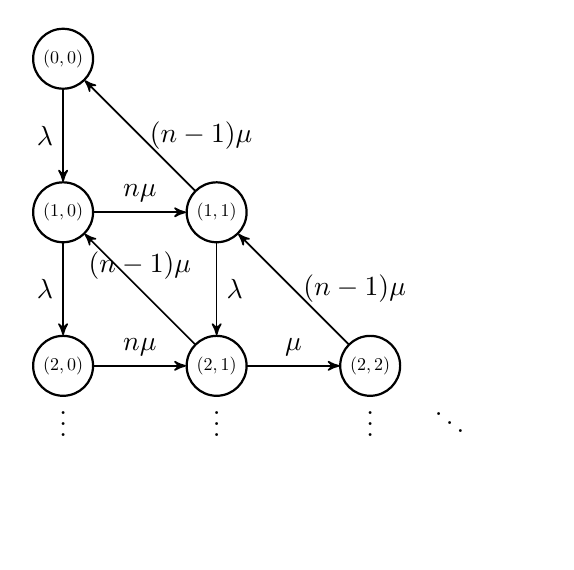
\begin{tikzpicture}[->, >=stealth', auto, semithick, node distance=3cm]
    \tikzstyle{every state}=[fill=white,draw=black,thick,text=black,scale=0.65]
    \node[state]    (0_0)					{$(0,0)$};
    \node[state]    (1_0)[below of=0_0]		{$(1,0)$};
    \node[state]    (1_1)[right of=1_0]		{$(1,1)$};
    \node[state]    (2_0)[below of=1_0]		{$(2,0)$};
    \node[state]    (2_1)[right of=2_0]		{$(2,1)$};
    \node[state]    (2_2)[right of=2_1]		{$(2,2)$};
%     \node[state]    (3_0)[below of=2_0]		{$(3,0)$};
%     \node[state]    (3_1)[right of=3_0]		{$(3,1)$};
%     \node[state]    (3_2)[right of=3_1]		{$(3,2)$};
%     \node[state]    (3_3)[right of=3_2]		{$(3,3)$};
    \node[state,draw=none]    (3_0)[below of=2_0]	{$ $};
    \node[state,draw=none]    (3_1)[right of=3_0]	{$ $};
    \node[state,draw=none]    (3_2)[right of=3_1]	{$ $};
    \node[state,draw=none]    (3_3)[right of=3_2]	{$ $};
    \path
    (0_0)
      edge	node[left]{$\lambda$}	(1_0)
    (1_0)
      edge	node[above]{$n\mu$}		(1_1)
      edge	node[left]{$\lambda$}	(2_0)
    (1_1)
      edge	node[right]{$(n-1)\mu$}	(0_0)
      edge	node[right]{$\lambda$}	(2_1)
    (2_0)
%       edge	node[left]{$\lambda$}	(3_0)
      edge  node[above]{$n\mu$}		(2_1)
      edge[draw=none]	node[auto=false,above]{$\vdots$}	(3_0)
    (2_1)
      edge	node[above]{$(n-1)\mu$}	(1_0)
      edge	node[above]{$\mu$}		(2_2)
%       edge	node[right]{$\lambda$}	(3_1)
      edge[draw=none]	node[auto=false,above]{$\vdots$}	(3_1)
    (2_2)
      edge	node[right]{$(n-1)\mu$}	(1_1)
%       edge  node[right]{$\lambda$}	(3_2)
      edge[draw=none]	node[auto=false,above]{$\vdots$}	(3_2)
      edge[draw=none]	node[auto=false,above]{$\ddots$}	(3_3);
%     (3_0)
%       edge	node[above]{$n\mu$}		(3_1)
%       edge[draw=none]	node[auto=false,above]{$\vdots$}	(4_0)
%     (3_1)
%       edge	node[above]{$(n-1)\mu$}	(2_0)
%       edge	node[above]{$\mu$}		(3_2)
%       edge[draw=none]	node[auto=false,above]{$\vdots$}	(4_1)
%     (3_2)
%       edge	node[above]{$\mu$}		(3_3)
%       edge	node[above]{$(n-1)\mu$}	(2_1)
%       edge[draw=none]	node[auto=false,above]{$\vdots$}	(4_2)
%     (3_3)
%       edge	node[right]{$(n-1)\mu$}	(2_2)
%       edge[draw=none]	node[auto=false,above]{$\vdots$}	(4_3)
%       edge[draw=none]	node[auto=false,above]{$\ddots$}	(4_4);
  \end{tikzpicture}
  \end{document}